\documentclass{article}

\usepackage[nonatbib, final]{neurips_2021}

\usepackage[utf8]{inputenc} % allow utf-8 input
\usepackage[T1]{fontenc}    % use 8-bit T1 fonts
\usepackage{hyperref}       % hyperlinks
\usepackage{url}            % simple URL typesetting
\usepackage{booktabs}       % professional-quality tables
\usepackage{amsfonts}       % blackboard math symbols
\usepackage{nicefrac}       % compact symbols for 1/2, etc.
\usepackage{microtype}      % microtypography
\usepackage{xcolor}         % colors
% own packages
\usepackage{amsmath}
\usepackage{multicol}
\usepackage{svg}
\usepackage[]{graphicx}
\usepackage{subfig}
\usepackage[square,numbers]{natbib}
\usepackage{stackengine}

\bibliographystyle{abbrvnat}
\setcitestyle{authoryear}

\newcommand\pef[1]{\hyperref[#1]{Section~\ref{#1}}}
\newcommand\fef[1]{\hyperref[#1]{Figure~\ref{#1}}}
\newcommand\tef[1]{\hyperref[#1]{Table~\ref{#1}}}

\title{Uncertainty Prediction - Seminar in AI}
\author{%
  Alexander Krauck \\
  Department of Machine Learning\\
  Johannes Kepler University Linz\\
  Upper Austria, Austria \\
  \texttt{alexander.krauck@gmail.com}
}
\date{August 2023}

\begin{document}

\maketitle

\section{What is Uncertainty in Machine Learning?}
Uncertainty is a complex topic in the field of machine learning and understanding it even more so. Generally when a machine learning model makes some prediction for an input, the question might arise how likely it is that this prediction is true. In particular, usually this problem is disected into two main parts. Firstly, it is asked, how certain is the model that it can make a reasonable prediction for this input data and secondly how sure is the model that the predicted solution is correct. Those two types of uncertainty are known as epistemic and aleatoric uncertainty respectively.

\subsection{Epistemic and Aleatoric Uncertainty} %needs rework
Even when predicting a distribution as an output, it is still not necissarely clear if the distribution is due to aleatoric or epistemic uncertainty. For example if the model outputs a very broad distribution, with very high variance, then one question that could arise is, if this strong uncertainty is due to lack of diverse training data or due to lack of information of the input x. For example epistemic uncertainty could be if the model has not seen any sample from this distribution yet. Then the model should possibly refer back to a prior distribution of the outputs. However, it might still be good if we, the users, somehow would know that this is due to lack of training data. I.e. possibly with this exact realization of x there might be a very tight distribution on the outcomes, however, the model does not know that and thus predicts a broad distribution as the prior. The other type of uncertainty is aleatoric. Here the model might have seen the input x before exactly, however, there still might be uncertainty because x might simply lack information that is required to predict y precisely. Thus we might still have a broad distribution, or a bimodal one. It is fundamental to identify whether or not aleatoric uncertainty is present in a system, since this is irreducible no matter how much training data the model receives. I believe in many systems this type of uncertainty is more present then we might think, especially for tabular data.

\section{Gaussian Process Neural Networks}
%TODO


\section{Bayesian Neural Networks + Bayesian Deep Learning}
\subsection{Basic Bayes}

The Bayes theorem is:
$$p(\boldsymbol{\omega} \mid \mathbf{X}, \mathbf{Y})=\frac{p(\mathbf{Y} \mid \mathbf{X}, \boldsymbol{\omega}) p(\boldsymbol{\omega})}{p(\mathbf{Y} \mid \mathbf{X}) }$$

Thereby it is important to note that we assume that certain variables are independent. For example $\omega$ and $\mathbf{X}$. The most difficult part of obtain this posterior $p(\boldsymbol{\omega} \mid \mathbf{X}, \mathbf{Y})$ is to get the model evidence $p(\mathbf{Y} \mid \mathbf{X})$. This is because for obtaining the model evidence we need to evaluate:
$$p(\mathbf{Y} \mid \mathbf{X})=\int p(\mathbf{Y} \mid \mathbf{X}, \boldsymbol{\omega}) p(\boldsymbol{\omega}) \mathrm{d} \boldsymbol{\omega}$$
which requires integrating the likelihood function over all possible realizations of $\omega$. This means we would need to input our samples into the likelihood function parameterized with every possible $\omega$ and take the average w.r.t. $\omega$. This is almost never possible analytically because it because intractable fast with complex parameterizations.

However, if we were able to determine $p(y^* \mid x^*, \mathbf{X}, \mathbf{Y})$, then we would be able to make many statements about the epistemic uncertainty of the neural network. The issue is, that for this we need
$$ p\left(\mathbf{y}^* \mid \mathbf{x}^*, \mathbf{X}, \mathbf{Y}\right) \approx \int p\left(\mathbf{y}^* \mid \mathbf{x}^*, \boldsymbol{\omega}\right) q_\theta^*(\boldsymbol{\omega}) \mathrm{d} \boldsymbol{\omega}=: q_\theta^*\left(\mathbf{y}^* \mid \mathbf{x}^*\right)$$
which can only be obtained by knowing the posterior or a good approximation $q_\theta^*\left(\mathbf{y}^*\right)$ thereof (Variational Inference). Using the theory of KL-divergence and ELBO, we can essentially replace integration due to marginalization in the evidence term by differentiation in the optimization procedure of gradient descent methods. This allows us to get estimates for the term that we want, at the cost of a more difficult and computationally expensive neural network optimization procedure than usually.

\section{Modeling aleatoric uncertainty}

In numerous machine learning tasks, it is advantageous to shift from a singular output to a spectrum of potential outputs, each accompanied by a measure of credibility, often expressed probabilistically. This is particularly pertinent when the mapping from input $\mathbf{x}$ to output cannot be established deterministically due to intrinsic aleatoric uncertainty. Consider a deterministic function $f: \mathbb{R}^d \rightarrow \mathbb{R}$. By sampling from a predefined distribution over $\mathbb{R}^d$ and applying $f$ to these samples, we can obtain a set of deterministically linked "targets". Subsequently, if we reduce the dimensionality of the input samples from $d$ to $k$ (where $k < d$), we are left with $\mathbb{R}^k$ samples. The challenge then becomes identifying an approximate function $f^*$ that accurately maps these reduced-dimension samples to the original outputs. This scenario encapsulates a significant portion of machine learning challenges. Often, the dimensionality reduction is minimal, allowing $f^*$ to approximate $f$ with negligible error. However, in instances where the reduction omits critical information, there may exist several viable predictions rather than a singular conclusive output. 

This is particularly evident in regression tasks where, for a given input, there may be several possible outputs. Such scenarios can be effectively modeled using multi-modal distributions, such as Gaussian mixture models, which allow for the representation of multiple potential outcomes with varying degrees of likelihood. By employing these advanced density networks, we can better accommodate the complexities and uncertainties inherent in real-world data.

A multitude of frameworks exist for addressing the prediction of multiple potential outcomes. Notable among these are \textbf{conformal prediction}, \textbf{conditional density estimation} (CDE), and \textbf{quantile regression}. Each of these frameworks are concerned about aleatoric uncertainty directly. It is worth noting that in contrast to Bayesian neural networks primarily address epistemic uncertainty, treating aleatoric uncertainty more or less as a by-product. The following subsections delve into these frameworks in detail.

\subsection{Conformal Prediction}
Conformal prediction assigns confidence measures to pairs of input samples and associated label sets $z = (\mathbf{x}, \{y_1, ..., y_n\})$. These confidence measures, or p-values, indicate the probability that the true label is within the predicted set. The nonconformity of each input-label pair—a measure of how "unusual" a prediction is—is typically calculated first. In contemporary machine learning, inductive conformal prediction is preferred over the traditional transductive approach. Inductive conformal prediction utilizes a trained model, such as a neural network, to compute nonconformity scores for potential outputs given an input $\mathbf{x}$, thereby constructing prediction sets with a specified confidence level, as formalized by \cite{Papadopoulos08}.

% Discussion on why softmax outputs do not equate to confidence measures %
\subsection{Conditional Density Estimation}
Conditional Density Estimation (CDE) encompasses a spectrum of techniques aimed at precisely characterizing $p(y \mid \mathbf{x})$, or more comprehensively, $p(y \mid \mathbf{x}, \mathbf{X}, \mathbf{Y})$. This predictive distribution is crucial, not only in the Bayesian framework and its manifestation in Bayesian neural networks, but also across a variety of applications where a full understanding of the distribution is necessary. In contrast to Bayesian methods, which typically approximate the predictive distribution through the estimation of its moments or the entropy to quantify epistemic uncertainty, CDE aspires to delineate the entire distribution, potentially capturing its intricate structure and potential multimodality. This distinction is significant: a complete depiction of the distribution, particularly its multimodal nature for a given data point, imparts a different level of insight compared to merely estimating a large target variance.

Among the prominent instances of CDE are Mixture Density Networks (MDNs). MDNs are designed to infer the parameters of a Gaussian mixture model based on input data, thereby predicting not just the mean and variance, but also the mixing coefficients for each component of the mixture. This approach translates into a robust framework capable of capturing the complex, potentially multimodal relationships between inputs and their corresponding targets.

The field is rich with methodologies, as evidenced by the work of \cite{rothfuss2019conditional}, which illustrates the expansive range of CDE techniques with neural networks. Recent contributions have particularly leveraged the power of normalizing flows, expounded upon by \cite{trippe2018conditional}, to model the conditional distributions with an unprecedented fidelity to their underlying complexity.

\subsection{Quantile Regression}
Quantile regression is an alternative approach that operates on the principle of the inverse cumulative distribution function (CDF). Regression models are trained to predict specific quantiles, essentially estimating fixed points on the inverse CDF of the target distribution given input data. This method allows for the construction of models targeting, for example, the 5th, 50th, and 95th percentiles, offering a granular perspective on the distribution's tails and central tendency.

The utility of quantile regression lies in its ability to illuminate the conditional distribution's structure, revealing asymmetries and tail behavior that average-based methods may obscure. While it bears an intuitive resemblance to credal sets, which provide a probabilistic guarantee that a set contains the true label, quantile regression lacks such formal assurances. The technique delineates boundaries within which certain proportions of the distribution lie, according to the estimated quantiles, without the probabilistic backing that credal sets are equipped with. This distinction is crucial, positioning quantile regression and credal sets as tools with unique merits and theoretical underpinnings.

% To augment the reader's understanding, a visual illustration of quantile regression's operation on the inverse CDF, or a discussion on its probabilistic interpretation, would be beneficial. %


\section{Datasets}
The datasets also visible in Table \ref{tab:dataset_comparison}, spanning various domains, have been widely recognized and employed in the machine learning community. Especially those datasets are popular for uncertainty prediction for regression tasks. The \textbf{Boston Housing} dataset, provides housing values in the suburbs of Boston, capturing factors such as crime rate, proximity to Charles River, and average number of rooms per dwelling. The \textbf{Concrete Compression Strength} dataset deals with the prediction of concrete strength, offering insights into its diverse ingredients and their interactions. \textbf{Energy Efficiency} dataset is centered on predicting the energy efficiency of buildings based on their architectural and construction features. \textbf{Kin8nm} is a synthetic dataset derived from a robotics application, whereas \textbf{Naval Propulsion} gives insights into the performance of naval ships based on parameters like turbine speed and compressor rate. The \textbf{Combined Cycle Power Plant} dataset is rooted in predicting the net hourly electrical energy output of a power plant. On a biological front, the \textbf{Protein Structure} dataset predicts the protein tertiary structure. The datasets on \textbf{Wine Quality Red} evaluates the quality of red wine based on physicochemical tests, and \textbf{Yacht Hydrodynamics} seeks to predict the hydrodynamic performance of sailing yachts from given parameters. Lastly, the \textbf{Year Prediction MSD} dataset is grounded in predicting the release year of a song from audio features. Fortunately, the accessibility of these datasets has been vastly simplified by the library called \texttt{alpaca-ml} which offers an integrated platform for their retrieval \cite{alpaca2023}. Originally, however those datasets are downloaded from various sources, with most of them originating from the UCI Machine Learning Repository by \cite{kelly2023uci} These datasets have commonly been leveraged to compare uncertainty prediction methods, serving as benchmarks in publications on the topic \cite{gal_dropout_2016, lakshminarayanan_ensembles_2017, hernandez2015probabilistic}.

\begin{table}
  \caption{Comparison of Different used Datasets}
  \label{tab:dataset_comparison}
  \centering
  \begin{tabular}{lrr}
    \toprule
    Dataset & \# Samples & \# Features \\
    \midrule
    Boston Housing & 506 & 13 \\
    Concrete Compression Strength & 1030 & 8 \\
    Energy Efficiency & 768 & 8 \\
    Kin8nm & 8192 & 8 \\
    Naval Propulsion & 11,934 & 16 \\
    Combined Cycle Power Plant & 9568 & 4 \\
    Protein Structure & 45,730 & 9 \\
    Wine Quality Red & 1599 & 11 \\
    Yacht Hydrodynamics & 308 & 6 \\
    Year Prediction MSD & 515,345 & 90 \\
    \bottomrule
  \end{tabular}
\end{table}



\section{Ideas}
1. I could use a dimensionality reduction method like PCA to reduce the input data of around 50 inputs to 1 input. Then I can just go along this principal component and use that as input. Moreover I can also use that for data analyzing, because I could simply plot the principal component of the samples against the model outputs. This might give a good idea about aleatoric uncertainty to some extent.


\section{Related Work}

\subsection{Quantification of Uncertainty with Adversarial Models}
\cite{schweighofer2023quantification} propose a novel technique for giving estimates on the uncertainty of a model. In particular, given a trained neural network as the reference model, they train a second adversarial network for each test point. The adversarial network has the objective to have a similar loss on the training set as the other model while having a very different loss on the test point. The intuition behind that is that if the reference model makes some prediction at the test point, and if other models (the adversaries) make different predictions while explaining the training data equally well, then one should be uncertain about the prediction. It is important to note that with the method of \cite{schweighofer2023quantification}, adversaries need to be trained for each individual test point. However, the reference network can be used as a starting point for the adversaries. %make sure that is all correct 

For representing the total predictive uncertainty, they provide two distinct definitions of total uncertainty. The distingtion can be a bit counter-intuitive. As they describe it, the first definition of uncertainty is valid when searching for the best parameters $\Tilde{w}$ out of the candidate parameters $\mathcal{W}$. In this case, they use the entropy over the marginalized predictive distribution $p(y \mid \mathbf{x}, \mathcal{D})$:


$$\mathrm{H}[p(\boldsymbol{y} \mid \boldsymbol{x}, \mathcal{D})] = \int_{\mathcal{W}} \operatorname{CE}(p(\boldsymbol{y} \mid \boldsymbol{x}, \tilde{\boldsymbol{w}}) ; p(\boldsymbol{y} \mid \boldsymbol{x}, \mathcal{D})) p(\tilde{\boldsymbol{w}} \mid \mathcal{D}) \mathrm{d} \tilde{\boldsymbol{w}}$$

$$= \underbrace{\int_{\mathcal{W}} \mathrm{H}[p(\boldsymbol{y} \mid \boldsymbol{x}, \tilde{\boldsymbol{w}})] p(\tilde{\boldsymbol{w}} \mid \mathcal{D}) \mathrm{d} \tilde{\boldsymbol{w}}}_{\text {aleatoric }}+\underbrace{\int_{\mathcal{W}} \operatorname{KL}(p(\boldsymbol{y} \mid \boldsymbol{x}, \tilde{\boldsymbol{w}}) \| p(\boldsymbol{y} \mid \boldsymbol{x}, \mathcal{D})) p(\tilde{\boldsymbol{w}} \mid \mathcal{D}) \mathrm{d} \tilde{\boldsymbol{w}}}_{\text {epistemic }}$$

In the other case, instead we assume a fixed given model $w$ and we want to infer how uncertain predictions under this model are. Moreover here we assume that the training set $\mathcal{D}$ is according to the true model.

$$
\int_W & \operatorname{CE}[p(\boldsymbol{y} \mid \boldsymbol{x}, \boldsymbol{w}), p(\boldsymbol{y} \mid \boldsymbol{x}, \tilde{\boldsymbol{w}})] p(\tilde{\boldsymbol{w}} \mid \mathcal{D}) \mathrm{d} \tilde{\boldsymbol{w}} \\
$$
$$
& \underbrace{\mathrm{H}[p(\boldsymbol{y} \mid \boldsymbol{x}, \boldsymbol{w})]}_{\text {aleatoric }}+\underbrace{\int_{\mathcal{W}} \mathrm{D}_{\mathrm{KL}}(p(\boldsymbol{y} \mid \boldsymbol{x}, \boldsymbol{w}) \| p(\boldsymbol{y} \mid \boldsymbol{x}, \tilde{\boldsymbol{w}})) p(\tilde{\boldsymbol{w}} \mid \mathcal{D}) \mathrm{d} \tilde{\boldsymbol{w}}}_{\text {epistemic }}
$$

Moreover, they separate the total predictive uncertainty into aleatoric and epistemic uncertainties. 

It is essential to notice that those definitions of uncertainty, while having a good mathematical foundation, are still just definitions and the resulting values when estimating uncertainties in those ways have to be interpreted with care. However, it is welcome to have definitions of uncertainty, that can be easily utilized to obtain uncertainty estimates in machine learning.

%insert mathematical foundation

\subsection{Dropout as a Bayesian Approximation: Representing Model Uncertainty in Deep Learning}

\cite{gal_dropout_2016} introduce a groundbreaking method for creating uncertainty estimates in deep learning. Expanding the mathematical foundation of bayesian neural networks, they successfully manage to represent any neural network that utilizes dropout, a very popular regularization technique, as bayesian neural networks. Moreover, this means that any such neural network also comes with a possibility to estimate uncertainty. Furthermore, they introduce a new method to make inference on neural networks that have been trained with Dropout: Monte-Carlo Dropout. Which essentially means that dropout is not only done during training but also during inference and the results are averaged in the end. 


\subsection{Aleatoric and Epistemic Uncertainty in Machine Learning: An Introduction to Concepts and Methods}
The work of \cite{hullermeier_aleatoric_2021} gives a new perspective on uncertainty handling and the probabilistic approach of machine learning methods. In particular, they showcase that probability theory, which is often perceived as the ultimate tool for handling uncertainty in machine learning methods, fails to capture all factors that define a machine learning problem. In particular the distinction between aleatoric and epistemic uncertainty is not possible with basic probability theory, but also require additional tools.

Moreover, they highlight that often in the machine learning field, people argue that the source of uncertainty is irrelevant. This might be true in some cases but in general this is not true, as can be seen in areas like active learning or in problems where a refusal-to-predict option exists for the model.

Another factor they introduce is that often a predictive set instead of a point prediction might be preferred. This in particular would be important for aleatoric uncertainty modeling, as with samples with a high uncertainty of that type can not be reasonably predicted with a single point.

Moreover, they discuss another distinction of uncertainties: Approximation uncertainty and model uncertainty. In this scenario we have a hypothesis space $\mathcal{H}$, which describes the set of models that we consider plausible or maybe also that might be easier to use. The approximation uncertainty then would be the difficulty to find the ideal model $f^* \in \mathcal{H}$, while the model uncertainty is the difference between the ideal model $f^*$ and the true underlying model that generated the data. Of course, as long as we are attempting to model a real world phenomenon with numeric methods, there will always be a model uncertainty, however the gap is small for a reasonable choice like a neural network usually. The major difficulty usually lies in identifying $f^*$. But, when taking a closer look, many decisions like the choice of hyperparameters or the initial parameters actually restrict $\mathcal{H}$ silently. So while of course neural network in theory are universal function approximators as first shown by \cite{HORNIK1989359}, those assumptive choices actually impose quite the restriction on the NN.

\subsubsection{Reducible vs. Irreducible Uncertainty}
An interesting thing to recognize is the connectedness of aleatoric and epistemic uncertainties. And even more intrestingly, when aleatoric uncertainty becomes epistemic and also vice versa. For example if we take the example from the work of \cite{hullermeier_aleatoric_2021} in figure \ref{fig:reducible_vs_irreducible}.

\begin{figure}[htbp]
  \centering
  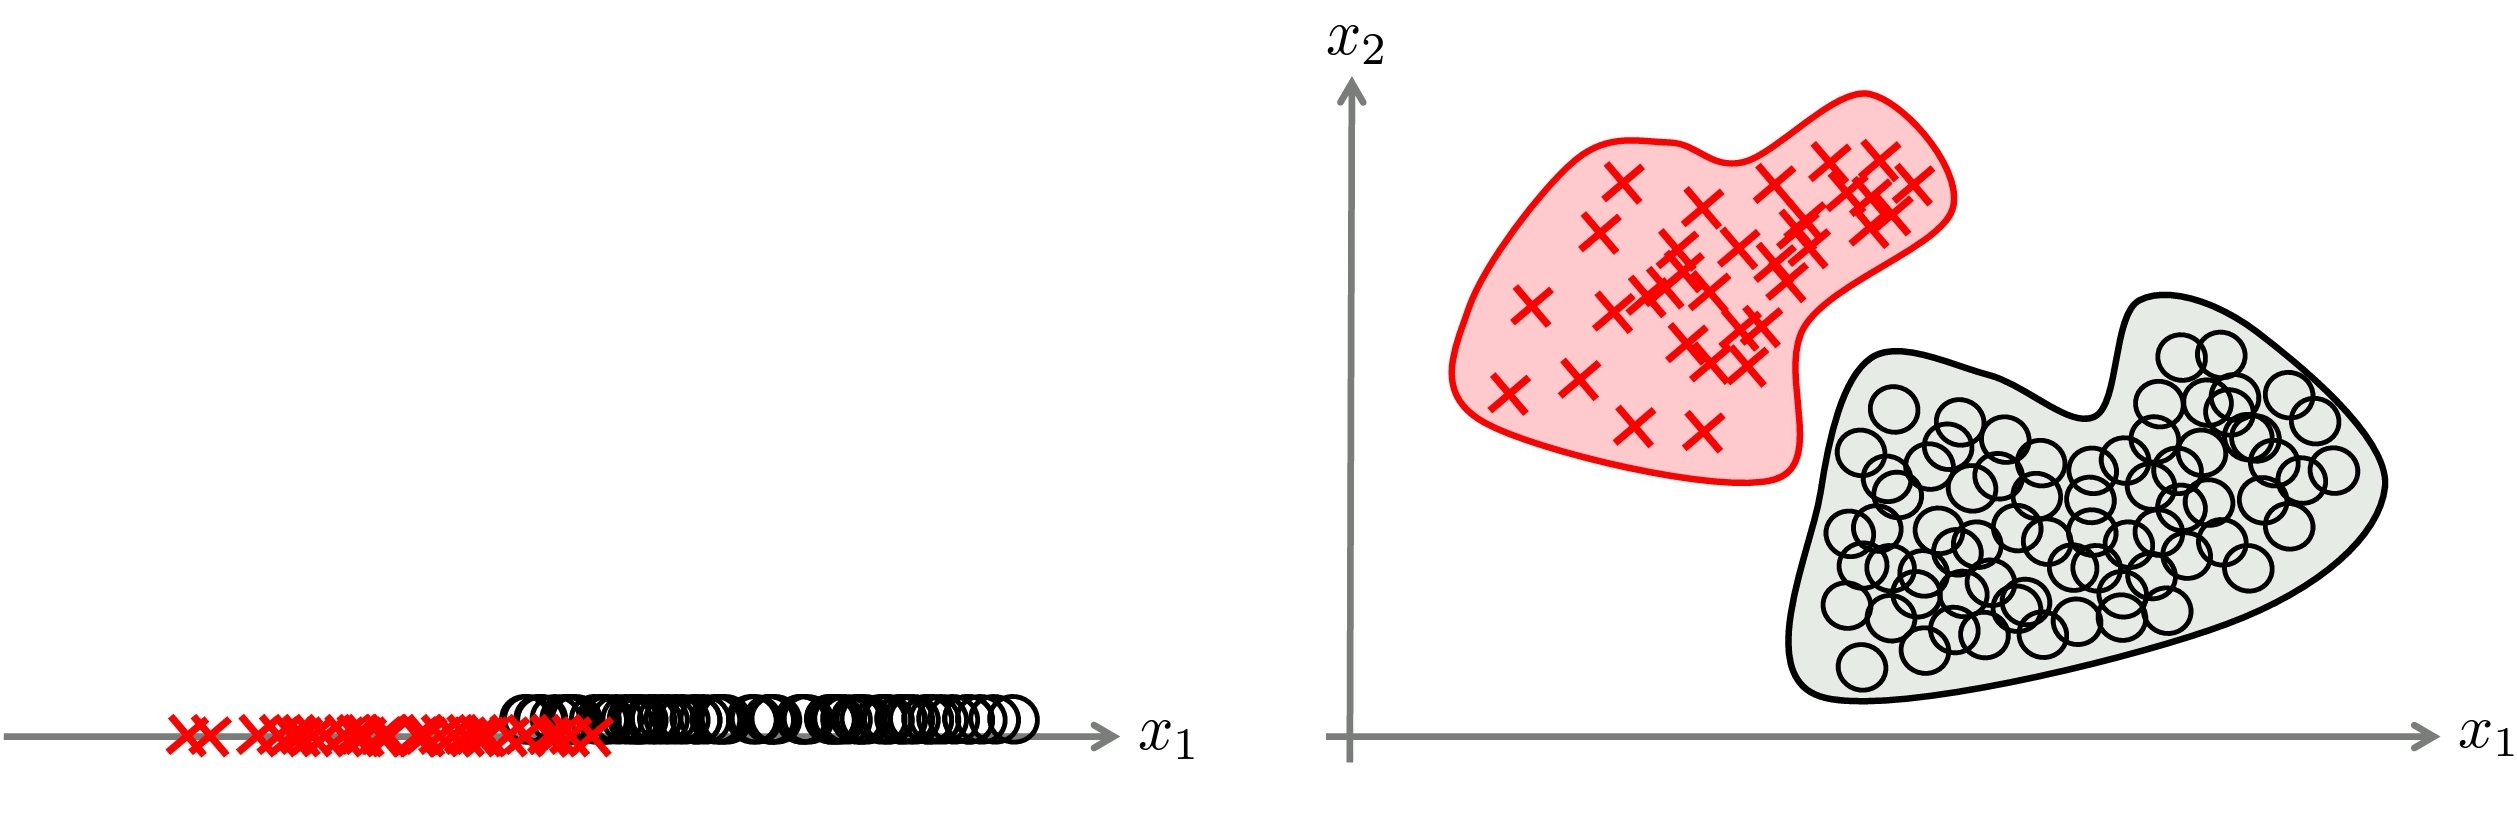
\includegraphics[width=\textwidth]{resources/reducible_vs_irreducible.jpg}
  \caption[More features separate labels]{On the left side, with only 1 feature, the data is not clearly separable by the lable, which means there is some aleatoric uncertainty. On the right hand side, the same data with another feature $x_2$ is added and now the data is clearly seperable by label. However, to find the "best possible" seperation on the left hand side we need less data than on the right hand side, meaning on the right hand side there is more epistemic uncertainty. Graphics taken from \cite{hullermeier_aleatoric_2021}}.
  \label{fig:reducible_vs_irreducible}
\end{figure}

\subsubsection{Learning without Assumptions is not Possible}
\cite{hullermeier_aleatoric_2021} highlight that a machine learning model can not be trained at all without specifying proper assumptions. With assumptions in this context all kinds of assumption around the model are meant. This means the model class, the parameters of the model (if it has some), the assumptions of the data, the assumptions of the training procedure (if it has one). One concept they use are \textbf{credal sets}. A credal set formalizes that if the assumptions that we need to make for the model are not unique/clear, then there also is not a single solution for the problem possibly, but multiple.

Taking neural networks as an example, consider the initialization of weights, which is typically drawn from a predefined probability distribution. This step, which might seem trivial, has profound implications on the network's eventual performance, due to the intricate optimization landscape of deep models. Given this, even a slight change in initialization can lead to a different final model, implying that our credal set — the set of plausible models given our current knowledge and assumptions — is vast. Another important example of a credal set of models are Bayesian Neural Networks (BNN). It is possible to interpret each realization of the BNN as an element of the credal set.
%% I NEED TO CHECKOUT "QUERYING CREDAL SETS" OR SO
%% ALSO IMPROVE THIS PART FUNDAMENTALLY

As \cite{wolpert_1996} gave the insight, if we increase the possible models to the set of all models, then when ignoring that this is intractable anyways, we see that any amount of data will not impact the outcome of the credal set. With other words, learning without assumptions is not possible.

\subsubsection{Difficulty Quantifying Uncertainty-Quality}

It is a rather difficult to do empirical evaluation for methods that predict uncertainty. Unlike for evaluating accuracy and such for classification/regression problems where labels are or can be provided, the inherent true quantification of uncertainty can be a highly ambiguous endeavor. A common way to still somehow quantify the usefulness of uncertainty methods is to use indirect approaches, where instead of directly predicting the uncertainty, instead the predictions of the model are somehow enhanced using the uncertainty estimates.

\begin{itemize}
    \item Accuracy-Rejection curves are a common way to do that. The background is that predictions where the model is more certain are usually expected to also be more accurate. If we now allow the model to refuse to make predictions for $p$\% of the samples where it is the least certain and also restrict the used metric on this restricted set, we can see the quality of the uncertainty prediction indirectly by the performance improvement of the model. The curve can be seen when modulating $p$.
\end{itemize}


\bibliography{references}

\end{document}


